\documentclass[12pt,a4paper]{article}
\usepackage[a4paper,top=1.5cm,bottom=1.7cm,left=1.9cm,right=1.6cm,footskip=0.9cm]{geometry}
\usepackage[T1]{fontenc}
\usepackage{amsmath}
\usepackage{newtxtext,newtxmath}
\usepackage{xcolor}
\usepackage{graphicx}
\usepackage{array,tabularx}
\usepackage{tikz}
\usetikzlibrary{calc,angles,quotes,arrows.meta}
\usepackage{fancyhdr}
\usepackage{enumitem}

\definecolor{qblue}{RGB}{0,0,230}

\pagestyle{fancy}
\fancyhf{}
\renewcommand{\headrulewidth}{0pt}
\fancyfoot[R]{\small Page \thepage/4 - Code 901}

\setlength{\parindent}{0pt}
\setlength{\parskip}{2pt}
\linespread{1.08}
\setlength{\lineskiplimit}{2pt}
\setlength{\lineskip}{3pt}

\newcommand{\Q}[1]{\textcolor{qblue}{\textbf{Question #1:}}}
\newcommand{\Ch}[1]{\textcolor{qblue}{\textbf{#1.}}}
% four choices on one line
\newcommand{\choicesFour}[4]{\par\hspace*{0.6cm}%
  \makebox[0.235\linewidth][l]{\Ch{A}~#1}%
  \makebox[0.235\linewidth][l]{\Ch{B}~#2}%
  \makebox[0.235\linewidth][l]{\Ch{C}~#3}%
  \makebox[0.235\linewidth][l]{\Ch{D}~#4}\par}
% two choices per line
\newcommand{\choicesTwo}[4]{\par\hspace*{0.6cm}%
  \makebox[0.47\linewidth][l]{\Ch{A}~#1}\makebox[0.47\linewidth][l]{\Ch{B}~#2}\par
  \hspace*{0.6cm}%
  \makebox[0.47\linewidth][l]{\Ch{C}~#3}\makebox[0.47\linewidth][l]{\Ch{D}~#4}\par}
\newcommand{\dotsfill}{\leavevmode\cleaders\hbox to 0.35em{\hss.\hss}\hfill\kern0pt}

\begin{document}

%================ HEADER ================
\noindent
{\fontsize{10.5}{13}\selectfont\begin{tabular}{@{}>{\centering\arraybackslash}p{0.35\linewidth}@{\hspace{0.01\linewidth}}p{0.64\linewidth}@{}}
\textbf{HAI PHONG DEPARTMENT OF}\par\textbf{EDUCATION AND TRAINING}
\par\vspace{8pt}
\fbox{\begin{minipage}{0.8\linewidth}\centering
\textbf{OFFICIAL TEST}\\ \textit{(There are 4 pages in this test)}
\end{minipage}}
&
\centering\textbf{EXAMINATION OF MATHEMATICS AND SCIENCE IN ENGLISH}\par
\textbf{ACADEMIC YEAR: 2025 -- 2026}\par\vspace{6pt}
\raggedright
\textbf{SUBJECT: MATHEMATICS}\par
\textbf{FOR: UPPER SECONDARY SCHOOL STUDENTS}\par
\textbf{Allotted time: 90 minutes}\par\vspace{4pt}
\hfill\fbox{\makebox[2.6cm]{\rule[-4pt]{0pt}{16pt}\textbf{Code 901}}}
\end{tabular}}

\vspace{10pt}
Candidate's full name:\makebox[0.52\linewidth]{\dotsfill}\ Identity number:\,\dotsfill
\par\vspace{2pt}
\noindent\rule{\linewidth}{0.4pt}
\vspace{4pt}

%================ PART I ================
\textbf{PART I. Multiple-choice questions (3,0 points).} \textit{Answer questions from 1 to 12. Choose no more than \textbf{ONE} option for each question.}

\Q{1} A family needs to drill a $50$-meter well to get water. They hire a well-drilling team to perform the work. Knowing the price of the first meter of drilling is $80\,000$ VND, from the second meter onwards, the price of each subsequent meter increases by $5\,000$ VND compared to the price of the previous meter. How much does the family have to pay to drill the well?
\choicesFour{$5\,250\,000$ VND.}{$10\,125\,000$ VND.}{$4\,000\,000$ VND.}{$4\,245\,000$ VND.}

\Q{2} Given a palabola $(P)\colon y=x^2+2mx+2m^2+m$. Let $S$ be the set of parameter $m$ such that the vertex of $(P)$ is lying on line $d\colon y=x+7$. The sum of the elements of $S$ is:
\choicesFour{$1$.}{$2$.}{$-2$.}{$-1$.}

\Q{3} In the coordinate plane $Oxy$, consider the ellipse $(E)\colon \dfrac{x^2}{a^2}+\dfrac{y^2}{b^2}=1$ $(a>b>0)$. $(E)$ passes through the point $M\left(\dfrac{3}{\sqrt5};\dfrac{4}{\sqrt5}\right)$ and $\widehat{F_1MF_2}=90^\circ$, with $F_1,F_2$ be two focal points of $(E)$.

\begin{center}
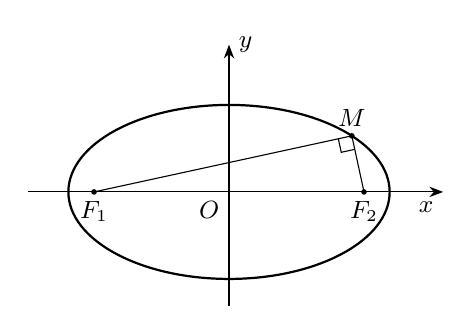
\begin{tikzpicture}[scale=0.85,font=\small]
  \def\a{2.4}\def\b{1.3}\def\c{2.017}
  \draw[-{Stealth[length=5pt]}] (-3,0) -- (3.2,0) node[below left] {$x$};
  \draw[-{Stealth[length=5pt]}] (0,-1.7) -- (0,2.2) node[right] {$y$};
  \draw[thick] (0,0) ellipse ({\a} and {\b});
  \coordinate (F1) at (-\c,0); \coordinate (F2) at (\c,0);
  \coordinate (M) at (1.835,0.838); \coordinate (O) at (0,0);
  \draw (F1) -- (M) -- (F2);
  \draw pic[draw,angle radius=5pt] {right angle=F1--M--F2};
  \fill (F1) circle (1.2pt) (F2) circle (1.2pt) (M) circle (1.2pt);
  \node[below] at (F1) {$F_1$}; \node[below] at (F2) {$F_2$};
  \node[above] at (M) {$M$}; \node[below left] at (O) {$O$};
\end{tikzpicture}
\end{center}

\hspace*{0.6cm}What is the value of $S=a^2+b^2$?
\choicesFour{$S=25$.}{$S=15$.}{$S=10$.}{$S=13$.}

\Q{4} In the coordinate plane $Oxy$, the circle $(C)$ has a diameter $AB$ with $A(1;1)$, $B(5;3)$. Which of the following is the equation of the circle $(C)$?
\choicesTwo{$(x+3)^2+(y+2)^2=5$.}{$(x-3)^2+(y-2)^2=20$.}{$(x-3)^2+(y-2)^2=5$.}{$(x+3)^2+(y+2)^2=20$.}

\Q{5} Randomly arrange $21$ students, including only one student named An and only one student named Chi, into three round tables with $6$, $7$ and $8$ seats. Each student takes one seat. The probability of the event ``An and Chi sit at the same table, but not next to each other'' is
\choicesFour{$\dfrac{43}{210}$.}{$\dfrac{23}{210}$.}{$\dfrac{1}{10}$.}{$\dfrac{21}{100}$.}

\newpage
\noindent\begin{minipage}[t]{0.56\linewidth}
\Q{6}\par
Mr. Smith has a quadrilateral plot of land $ABCD$, where $AB=8$ m, $BC=7$ m, $AD=3$ m, $\widehat{ABC}=40^\circ$, $\widehat{BAD}=100^\circ$ (as seen in the figure). What is the minimum amount of money Mr. Smith has to pay to fence around the plot of land, knowing that each meter of fence costs \$$1.8$? (unit: \$, round to the tenths).\par
\hspace*{0.6cm}\Ch{A} $38.7$.\par
\hspace*{0.6cm}\Ch{B} $39.1$.\par
\hspace*{0.6cm}\Ch{C} $39.3$.\par
\hspace*{0.6cm}\Ch{D} $38.5$.
\end{minipage}\hfill
\begin{minipage}[t]{0.42\linewidth}
\vspace{2pt}\centering
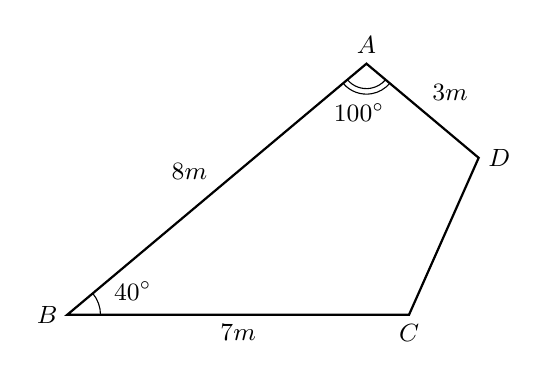
\begin{tikzpicture}[scale=0.62,font=\small]
  \coordinate (B) at (0,0); \coordinate (C) at (7,0);
  \coordinate (A) at (6.128,5.142); \coordinate (D) at (8.426,3.214);
  \draw[thick] (A) -- (B) -- (C) -- (D) -- cycle;
  \node[left] at (B) {$B$}; \node[below] at (C) {$C$};
  \node[above] at (A) {$A$}; \node[right] at (D) {$D$};
  \draw pic["$40^\circ$",draw,angle radius=12pt,angle eccentricity=2.1] {angle=C--B--A};
  \draw pic[draw,angle radius=9pt] {angle=B--A--D};
  \draw pic[draw,angle radius=11pt] {angle=B--A--D};
  \node at ($(A)+(-0.15,-1.0)$) {$100^\circ$};
  \node[above left] at ($(A)!0.5!(B)$) {$8m$};
  \node[below] at ($(B)!0.5!(C)$) {$7m$};
  \node[above right] at ($(A)!0.5!(D)$) {$3m$};
\end{tikzpicture}
\end{minipage}

\Q{7} Given a function $f(x)=ax^2+bx+c$ $(a\neq0)$ whose graph is shown below.

\par\vspace{2pt}\centerline{%
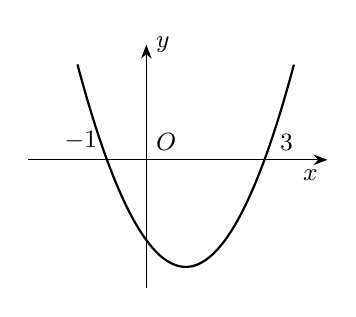
\begin{tikzpicture}[xscale=0.5,yscale=0.34,font=\small]
  \draw[-{Stealth[length=5pt]}] (-3,0) -- (4.6,0) node[below left] {$x$};
  \draw[-{Stealth[length=5pt]}] (0,-4.8) -- (0,4.3) node[right] {$y$};
  \draw[thick,domain=-1.75:3.75,samples=100] plot (\x,{\x*\x-2*\x-3});
  \node[above left] at (-1,0) {$-1$};
  \node[above right] at (0,0) {$O$};
  \node[above right] at (3.15,0) {$3$};
\end{tikzpicture}}\par\vspace{2pt}

\hspace*{0.6cm}The number of solutions in the interval $(0;4\pi)$ of the equation $f(2\cos x)=0$ is:
\choicesFour{$4$.}{$2$.}{$0$.}{$6$.}

\Q{8} Given the prism $ABC.A'B'C'$. Let $M,P$ be the midpoints of the edges $BC$, $A'C'$, respectively. Which of the following planes is the line $MP$ parallel to?
\choicesFour{$(ABB'A')$.}{$(AB'C')$.}{$(AB'C)$.}{$(A'BC')$.}

\Q{9} Given a pyramid $S.ABCD$ with a parallelogram base $ABCD$. Let $M,P$ be the midpoints of edges $SA$ and $SC$, respectively. Let $N$ be the point lying on edge $SB$ such that $\dfrac{SN}{SB}=\dfrac{5}{8}$. Let $Q$ be the intersection point of edge $SD$ and plane $(MNP)$. The ratio $\dfrac{QS}{QD}$ is:
\choicesFour{$\dfrac{10}{13}$.}{$\dfrac{5}{7}$.}{$\dfrac{6}{7}$.}{$\dfrac{12}{13}$.}

\Q{10} Given the line $(d)$ passes through $M(6;2)$. Let $A,B$ be the intersections of line $(d)$ with graph of the funtions $y=\log_{\sqrt2}x$ and $y=\log_{\frac12}x$, respectively. Suppose $M$ is the midpoint of segment $AB$, what is the distance from $O(0;0)$ to line $(d)$?
\choicesFour{$2\sqrt5$.}{$4\sqrt5$.}{$3\sqrt2$.}{$4\sqrt2$.}

\Q{11} Given the sequence $(u_n)$ satisfying $\begin{cases} u_1=5\\ u_{n+1}=u_n+3n+2,\ \forall n\in\mathbb{N}^*\end{cases}$.

\hspace*{0.6cm}What is the value of $\displaystyle\lim\frac{u_n}{2n^2-3n+2}$?
\choicesFour{$\dfrac12$.}{$\dfrac34$.}{$1$.}{$\dfrac32$.}

\noindent\begin{minipage}{\linewidth}
\Q{12} Given the grouped data regarding the weight (unit: gram) of potatoes as follows:\par
{\renewcommand{\arraystretch}{1.15}
\begin{tabularx}{\linewidth}{|l|*{5}{>{\centering\arraybackslash}X|}}
\hline
\textbf{Weight} & $[70;80)$ & $[80;90)$ & $[90;100)$ & $[100;110)$ & $[110;120)$\\ \hline
\textbf{Frequency} & $3$ & $6$ & $12$ & $6$ & $3$\\ \hline
\end{tabularx}}\par
\hspace*{0.6cm}The first quartile of this grouped data is:
\choicesFour{$Q_1=86.5$.}{$Q_1=85.5$.}{$Q_1=86.75$.}{$Q_1=87.5$.}
\end{minipage}

%================ PART II ================
\newpage
\textbf{PART II. Short-answer questions (7.0 points).} \textit{Give short answers to questions from 1 to 10.}\par
\textbf{\underline{Note:} Round the result up by the last operation in the math problems.}

\Q{1} In bad weather, a fishing vessel at position $M$ sends a distress signal. Two signal receiving stations $A$ and $B$ are located along the coast and are $100$ kilometers apart. The radio signal from vessel $M$ reaches station $A$ $0.2\times10^{-3}$ seconds earlier than it reaches station $B$. The speed of radio signal transmission in the air is $300\,000$ km/s. Using radar, it is determined that vessel $M$ is at a distance of $40$ kilometers from the line connecting the two stations. A rescue boat departs from port $K$, which is the midpoint of the segment connecting two stations $A$ and $B$.\par
\hspace*{0.6cm}What is the distance from port $K$ to vessel $M$? (Unit: km, round the result to the tenths)

\par\vspace{3pt}\noindent
\begin{minipage}[b]{0.46\linewidth}\centering
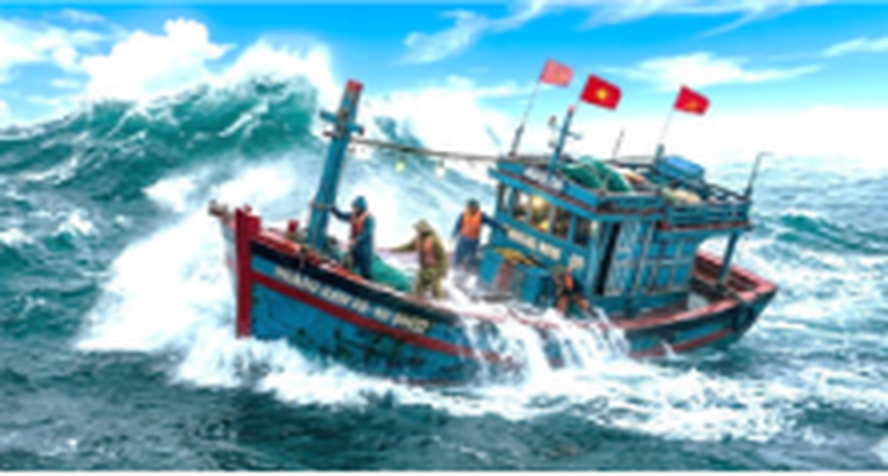
\includegraphics[width=0.85\linewidth]{boat.png}
\end{minipage}\hfill
\begin{minipage}[b]{0.5\linewidth}\centering
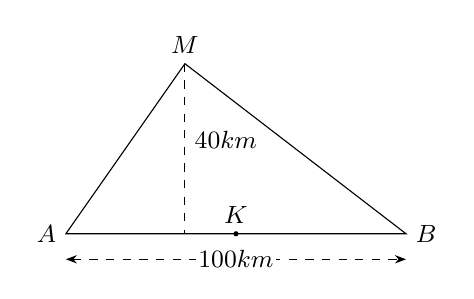
\begin{tikzpicture}[scale=0.72,font=\small]
  \coordinate (A) at (0,0); \coordinate (B) at (6,0); \coordinate (K) at (3,0);
  \coordinate (M) at (2.1,3.0); \coordinate (H) at (2.1,0);
  \draw (A) -- (M) -- (B) -- cycle;
  \draw[dashed] (M) -- (H);
  \fill (K) circle (1.3pt);
  \node[left] at (A) {$A$}; \node[right] at (B) {$B$};
  \node[above] at (M) {$M$}; \node[above] at (K) {$K$};
  \node[right] at ($(M)!0.45!(H)$) {$40km$};
  \draw[dashed,{Stealth[length=4pt]}-{Stealth[length=4pt]}] (0,-0.45) -- (6,-0.45);
  \node[fill=white,inner sep=1pt] at (3,-0.45) {$100km$};
\end{tikzpicture}
\end{minipage}
\par\vspace{3pt}

\Q{2} Given pyramid $S.ABCD$ with base $ABCD$ being a parallelogram. Let $G$ be the centroid of triangle $ABC$ and $E$ be a point on edge $SA$ satisfying $SE=\dfrac{m}{n}SA$ with $\dfrac{m}{n}$ being a simplified fraction. Given that $GE$ is parallel to plane $(SCD)$. What is the product of $m$ and $n$?

\Q{3} How many six-digit natural numbers are there such that the product of their digits is equal to $1400$?

\Q{4} Let $x$ and $y$ be non-negative real numbers satisfying the system of inequations\par
\hspace*{0.6cm}$\begin{cases}3x+y\le21\\ x+y\le9\\ x+4y\le24\end{cases}$\par
\hspace*{0.6cm}What is the maximum value of the expression $F(x;y)=50x-30y$?

\Q{5} $200$ male students and $200$ female students participate in pair dancing. There are $200$ yellow cards sequentially numbered $5,8,11,14,17,\ldots$ and $200$ blue cards sequentially numbered $3,7,11,15,19,\ldots$. The organizers ask each female student to take one yellow card and each male student to take one blue card. A male and a female will dance together if they hold identical numbers. How many dancing pairs will there be?

\begin{minipage}[t]{0.64\linewidth}
\Q{6} Two apartment buildings are $HK=20$ m apart. A camera is installed at $C$ on the roof of Building 2 to observe Building 1 (as seen in the figure). The heights of the two buildings are $BH=24$ m and $CK=32$ m. $A$ and $B$ are the lowest and highest points observable such that $\dfrac{BA}{BH}=\dfrac56$. Angle $\widehat{ACB}$ is the camera's angle of view. Given $\tan\widehat{ACB}=\dfrac{a}{b}$ $\Big(\dfrac{a}{b}$ is a simplified fraction$\Big)$. What is the value of $a+b$?
\end{minipage}\hfill
\begin{minipage}[t]{0.33\linewidth}
\vspace{0pt}\centering
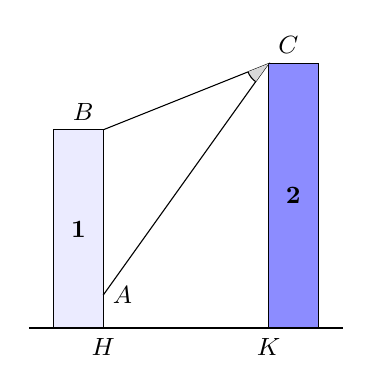
\begin{tikzpicture}[scale=0.105,font=\small]
  \coordinate (H) at (0,0); \coordinate (K) at (20,0);
  \coordinate (B) at (0,24); \coordinate (C) at (20,32); \coordinate (A) at (0,4);
  \fill[blue!8] (-6,0) rectangle (0,24);  \draw (-6,0) rectangle (0,24);
  \fill[blue!45] (20,0) rectangle (26,32); \draw (20,0) rectangle (26,32);
  \draw[thick] (-9,0) -- (29,0);
  \draw (B) -- (C) -- (A);
  \draw pic[draw,fill=gray!30,angle radius=8pt] {angle=B--C--A};
  \node at (-3,12) {\textbf{1}}; \node at (23,16) {\textbf{2}};
  \node[above left] at (B) {$B$}; \node[above right] at (C) {$C$};
  \node[right] at (A) {$A$};
  \node[below] at (H) {$H$}; \node[below] at (K) {$K$};
\end{tikzpicture}
\end{minipage}

\newpage
\Q{7} Given the function $f(x)=\begin{cases}\dfrac{\sqrt{1+ax^2}-bx-2}{4x^3-3x+1} & \text{when } x\neq\dfrac12\\[10pt] \dfrac{c}{2} & \text{when } x=\dfrac12\end{cases}$ $(a,b,c\in\mathbb{Z})$.\par
\hspace*{0.6cm}Knowing funtion $f(x)$ is continuous at $x=\dfrac12$, what is the value of $S=abc$?

\Q{8} Given a pyramid $S.ABCD$ with base $ABCD$ being a rhombus of side length $2\sqrt3$, $SA=2$, $SB=SC=SD=2\sqrt3$. A plane $(P)$ passes through $S$ and is perpendicular to $AD$, intersecting $AD$ and $BC$ at $M$ and $N$, respectively. Compute the area of triangle $SMN$. (Round the result to the hundredths)

\Q{9} Let the real numbers $a,b,c$ be greater than $1$ and satisfy
\[\log^2_{\sqrt a}b+\left(\log_b c-1\right)\log_b\sqrt c+\log_a\frac{c^3}{b}=0\]
\hspace*{0.6cm}What is the value of $P=\dfrac{4}{\log_b a}+\log_b(bc)$?

\Q{10} Given the set $A=\{1,2,3,\ldots,90\}$. Randomly choose a $3$-element subset of $A$ such that the sum of its elements is $91$. Let $P$ be the probability of the event ``3 elements of the chosen subset form a geometric sequence''. What is the value of $\dfrac1P$?

\vspace{14pt}
\begin{center}-{}-{}-{}-{}-{}-{}-{}-{}-{}-{}-{} The end -{}-{}-{}-{}-{}-{}-{}-{}-{}-{}\end{center}

\vfill
Invigilator No.1:\makebox[0.33\linewidth]{\dotsfill}\hspace{1em}Invigilator No.2:\dotsfill

\end{document}
